\section{Démarche Expérimentale}

\paragraph{Mesure de l'efficacité}
Afin de déterminer expérimentalement l'efficacité du moteur de Stirling, trois méthodes sont utilisées pour calculer la puissance \(P_m\) du moteur. L'efficacité expérimentale \(\eta\) est alors donnée par la puissance de sortie du moteur sur la puissance d'entrée \(\phi_2\):

\begin{equation}
    \eta = \frac{P_m}{\phi_2}
    \label{eq:efficacite}
\end{equation}

où \(\phi_2\) est la puissance de la source chaude, provenant d'un filament chauffé par effet Joule. Sa puissance est donnée par \(\phi_2 = UI\), avec \(U\) la tension et \(I\) l'intensité du courant dans le filament.

Le dispositif expérimental à la \autoref{fig:montage} est connecté à un système analogique permettant de tracer le diagramme PV du cycle de Stirling, en faisant bouger un petit miroir permettant de projeter le laser sur une feuille. La première méthode consiste à trouver le travail \(W\) effectué au cours d'un cycle en trouvant l'aire sous la courbe. Avec \(\omega\) la vitesse angulaire du volant d'inertie, la puissance est donnée par 
\begin{equation}
    P_\textrm{m,PV} = c A \frac{\omega}{2 \pi}
    \label{eq:pm_pv}
\end{equation}
où \(c\) est une constante trouvée avec l'étalonnage du graphique et \(A\) est l'aire sous la courbe.

%% Pour bien placer le montage
\begin{wrapfigure}{L}{0.5\linewidth}
    \centering
    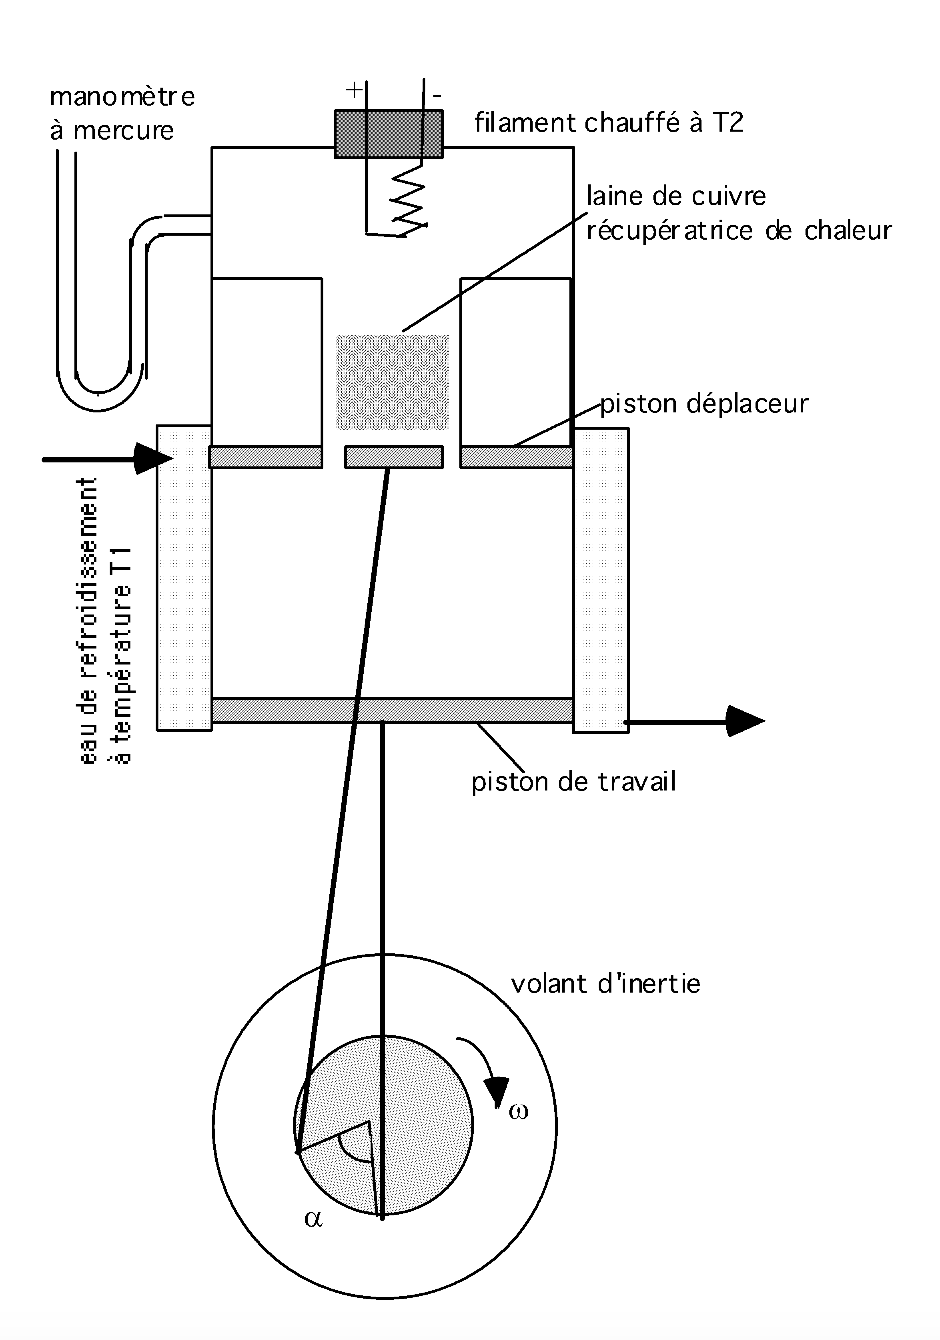
\includegraphics[width=\linewidth]{figures/montage.png}
    \caption{Schéma du montage du moteur Stirling \cite{notice}}
    \label{fig:montage}
    \vspace{1cm}
\end{wrapfigure}

Un disque de freinage, composé de plusieurs aimants placés à équidistance sur le bord du disque, permet de freiner le volant d'inertie en utilisant l'induction magnétique. La distance entre le disque et le volant peut être variée. La force sur le disque de freinage est mesurée sur le bord du disque par un dynamomètre accroché à la verticale. Le moment des forces sur le disque est alors donné par
\begin{equation}
    ||\vec{M}|| = ||\vec{R} \times \vec{F}|| = RF \cos{\alpha}
    \label{eq:couple}
\end{equation}
où \(\vec{R}\) est le vecteur de norme \(R\) entre le centre du disque et le point d'application de la force \(F\) et \(\alpha\) est l'angle entre le point du disque où la force est mesurée et l'horizontale. La puissance mécanique est alors donnée par
\begin{equation}
    P_\textrm{m,frein} = ||\vec{M}||\frac{\omega}{2 \pi} = F R \frac{\omega}{2 \pi} \cos{\alpha}
    \label{eq:pm_frein}
\end{equation}
où \(\omega\) est la vitesse angulaire du volant d'inertie en \si{\radian\per\second} \cite{chadsermet}. Le moment des forces est ici égal au couple mécanique: \(||\vec{M}|| = C\).

Enfin, la dernière méthode considère simplement la différence des flux chauds \(\phi_2\) et froids \(\phi_1\). Le flux froid \(\phi_1\) correspond au flux de chaleur évacué par le système de refroidissement à eau.
\begin{equation}
    \phi_1 = C_\textrm{m,eau} \rho_\textrm{eau} D \Delta T
\end{equation}
où \(C_\textrm{m,eau} = (4179.6 \pm 0.1)\) \si{\joule\per\kelvin\per\kilo\gram} est la capacité thermique massique de l'eau \cite{proprietes-eau}, \mbox{\(\rho_\textrm{eau} = (999.9 \pm 0.1)\) \si{\kilo\gram\per\meter\cubed}} est la masse volumique de l'eau \cite{proprietes-eau}, \(D\) est le débit d'eau et \(\Delta T\) est la différence de température entre l'entrée et la sortie d'eau. La puissance correspond alors à la différence de flux:

\begin{equation}
    P_\textrm{m,chaleur} = \phi_2 - \phi_1 = UI - C_\textrm{m,eau} \rho_\textrm{eau} D \Delta T
    \label{eq:pm_chaleur}
\end{equation}

\begin{wrapfigure}{R}{0.42\linewidth}
    \centering
    %% j'adore le latex (non)
    \vspace{-1cm}
    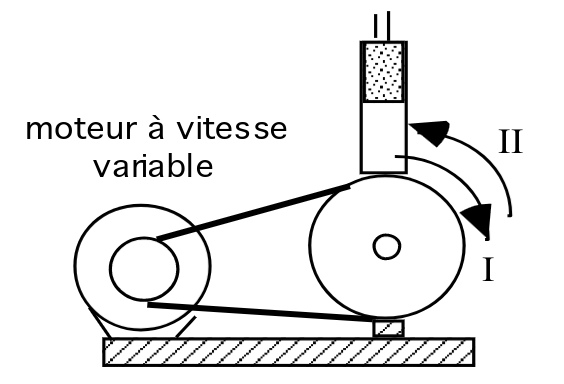
\includegraphics[width=\linewidth]{figures/machine-frigo.png}
    \caption{Schéma du moteur de Stirling comme machine frigorifique \cite{notice}}
    \label{fig:machine_frigo}
    \vspace{-0.5cm}
\end{wrapfigure}

\paragraph*{Machine frigorifique}
Lors de cette expérience le fonctionnement du cycle de Stirling en machine frigorifique est le point d'intérêt. Il s'obtient en tournant l'arbre de rotation à l'aide d'un moteur externe dont il est possible de mesurer la puissance fournie \(P_{moteur}\) par mesure de sa tension et de son courant d'entrée. Il est important de faire tourner dans ce cas le cycle dans le même sens que lors du fonctionnement moteur afin d'évacuer la chaleur de la tête de mesure, cela correspond au sens de rotation I dans la \autoref{fig:machine_frigo}. Pour minimiser les échanges de chaleur avec l'environnement, qui viendraient perturber la mesure de l'extraction de chaleur par le cycle frigorifique, un filament de compensation de température doit être présent dans la chambre refroidie \cite{notice}. Il doit être réglé pour maintenir une température similaire à celle extérieure. Afin de calculer le rendement de ce cycle frigorifique par l'\autoref{eq:rend-frigo} les tensions et intensités d'entrée du filament sont mesurées. La puissance \(P_{filament}\) ainsi obtenue est celle qui vient exactement compenser le flux de chaleur \(\phi_2\) évacué par la machine frigorifique pour maintenir une température constante avec \(P_{filament} = \phi_2\).
